% Generated by ICLR_Q4.py from experiment_logs_Q4 -- Drone4D_x0set: Reach-avoid prob.
% Shaded band = min/max over seeds; line = median over seeds.
% Picture width is exactly \linewidth. Requires \usepackage{pgfplots}.
% Bounds below ymin lie outside the axis range and are clipped.
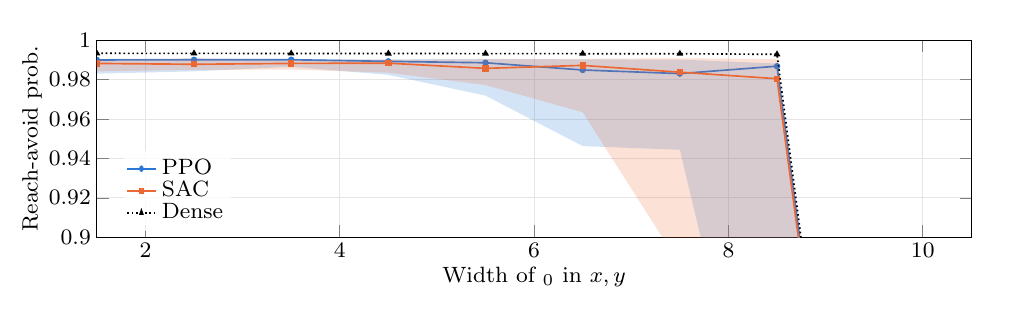
\begin{tikzpicture}[baseline=(current axis.south)]
\definecolor{q4ppo}{RGB}{42,120,214}
\definecolor{q4sac}{RGB}{235,104,52}
\definecolor{q4dense}{RGB}{0,0,0}
\begin{axis}[
    scale only axis, width=\linewidth-25pt-4pt, height=2.5cm,
    xlabel={Width of $\X_0$ in $x,y$},
    ylabel={Reach-avoid prob.}, ylabel style={align=center},
    xmin=1.5, xmax=10.5, xtick={2,4,6,8,10},
    ymin=0.9, ymax=1,
    grid=major, grid style={gray!20}, clip marker paths=true,
    label style={font=\footnotesize}, tick label style={font=\footnotesize, inner sep=2pt},
    xlabel shift=-2pt, ylabel shift=-3pt,  % labels close to the tick labels
    legend pos=south west, legend cell align=left,
    legend style={font=\footnotesize, draw=none, fill=white, fill opacity=0.8, text opacity=1,
        inner sep=1pt, row sep=-3pt},
    legend image post style={xscale=0.6},
]
% PPO: 5 seeds per X0 span
\addplot[draw=none, fill=q4ppo, fill opacity=0.2, forget plot] coordinates {(1.5,0.983048) (2.5,0.984237) (3.5,0.986539) (4.5,0.982462) (5.5,0.971915) (6.5,0.946265) (7.5,0.944395) (8.5,0.737561) (9.5,0.579626) (10.5,6.47648e-05) (10.5,6.60345e-05) (9.5,0.615019) (8.5,0.98822) (7.5,0.990203) (6.5,0.990298) (5.5,0.99061) (4.5,0.990302) (3.5,0.990244) (2.5,0.990682) (1.5,0.99063)} -- cycle;
\addplot[q4ppo, semithick, mark=*, mark size=0.85pt] coordinates {(1.5,0.990029) (2.5,0.990095) (3.5,0.990135) (4.5,0.989302) (5.5,0.988594) (6.5,0.984926) (7.5,0.983088) (8.5,0.986856) (9.5,0.614088) (10.5,6.59718e-05)};
\addlegendentry{PPO}
% SAC: 5 seeds per X0 span
\addplot[draw=none, fill=q4sac, fill opacity=0.2, forget plot] coordinates {(1.5,0.984227) (2.5,0.984956) (3.5,0.98514) (4.5,0.983544) (5.5,0.977283) (6.5,0.963407) (7.5,0.885949) (8.5,0.224063) (9.5,0.010669) (10.5,0) (10.5,6.60885e-05) (9.5,0.615674) (8.5,0.99041) (7.5,0.990888) (6.5,0.990597) (5.5,0.990402) (4.5,0.990131) (3.5,0.990286) (2.5,0.990748) (1.5,0.990256)} -- cycle;
\addplot[q4sac, semithick, mark=square*, mark size=0.85pt] coordinates {(1.5,0.988244) (2.5,0.987828) (3.5,0.988263) (4.5,0.988385) (5.5,0.985761) (6.5,0.987255) (7.5,0.983802) (8.5,0.980507) (9.5,0.613256) (10.5,6.57905e-05)};
\addlegendentry{SAC}
% Dense (single deterministic run per X0 span)
\addplot[q4dense, semithick, mark=triangle*, mark size=0.85pt, densely dotted, mark options={solid}] coordinates {(1.5,0.993398) (2.5,0.993361) (3.5,0.993323) (4.5,0.993289) (5.5,0.993252) (6.5,0.993215) (7.5,0.993182) (8.5,0.992878) (9.5,0.616133) (10.5,6.6147e-05)};
\addlegendentry{Dense}
\end{axis}
% Fix the bounding box to exactly \linewidth wide: the axis box plus the label margins
\path (current axis.south west |- current bounding box.south) ++(-25pt,0) coordinate (q4sw)
      (current axis.north east |- current bounding box.north) ++(4pt,0) coordinate (q4ne);
\pgfresetboundingbox
\useasboundingbox (q4sw) rectangle (q4ne);
\end{tikzpicture}%
